\section{Mechanism-Informed Consequence Surrogate}
\label{sec:surrogate}

The final factors of Equation~\eqref{eq:consequence} --- the probability of
significant spread and of evacuation failure given ignition --- depend on physical
building geometry and occupant behaviour that no public register records directly.
In place of real geometry, we represent each building as a synthetic
\emph{archetype graph}: nodes are typed rooms, corridors, stairs, lobbies and
exits, and edges carry a compartmentation-barrier type (open, internal door, fire
door, compartment wall) and a traversal length. Seven families cover the
minimum-viable-product (MVP) scope --- detached and terraced houses, low-rise and
high-rise purpose-built flats, HMO,
care-home-like wing, and mixed-use residential-over-commercial --- parameterised by
storeys, occupant count, mobility-impaired fraction, and number of exits.

Fire develops as a stochastic process on the graph. An ignition (located by
room-kind weights derived from the dwelling-fires data, kitchens dominant) is most
often minor and self-limits at the room of origin; a developing fire spreads by
lognormal smoke and flame crossing times, gated by the barrier states, until the
earliest of occupant control, fuel-limited burnout, or fire-service suppression.
Detection depends on alarm state and on whether occupants are asleep; evacuation is
simulated per occupant with heterogeneous awareness and pre-movement times, walking
the shortest currently-tenable route to an exit and re-routing as nodes become
untenable. Evacuation failure is a route cut before egress. The construction is a
deliberately transparent stochastic caricature calibrated to plausible orderings
and magnitudes, not a CFD or Fire Dynamics Simulator (FDS) replacement; every
parameter is declared with a
provenance tag in a single assumptions registry, and the physical orderings it
encodes --- better compartmentation and working detection lower every consequence
probability, night and mobility impairment raise evacuation failure --- are what
make it \emph{mechanism-informed and physically constrained} rather than a black-box fit
\citep{yarmohammadian2025pism,yildiz2025ml}.

Algorithm~\ref{alg:sim} states one Monte Carlo iteration exactly as implemented
(\texttt{src/sim/fire.py} and \texttt{evacuation.py}); a cell probability is the
sample mean of the recorded outcome over $N$ such iterations
(\texttt{run\_experiments.py}, $N=10{,}000$).

\begin{algorithm}[htbp]
\caption{One iteration of the building fire--outcome simulator (one ignition).}
\label{alg:sim}
\small
\begin{algorithmic}[1]
\State \textbf{Input:} archetype graph $G=(V,E)$ (typed nodes; edges with barrier
class $b$ and length $\ell$); scenario (alarm $\in\{$none, present-not-working,
working$\}$, time $\in\{$day, night$\}$); RNG.
\State $\text{ignition} \gets$ node sampled $\propto$ room-kind ignition weights
(kitchen-dominant; exits excluded) \Comment{\texttt{sample\_ignition}}
\State $(r_0,f_0) \gets$ room and floor of the ignition node
\For{each edge $(u,v)\in E$ with barrier $b$}
  \State $p_{\text{open}} \gets$ baseline open-probability of $b$;
  \textbf{if} night and $b=$ internal door \textbf{then} $p_{\text{open}}
  \mathrel{\times}= 0.35$
  \State $\text{open} \gets [\,\mathcal{U}(0,1) < p_{\text{open}}\,]$; pick smoke,
  flame medians $s_b,f_b$ for that open/closed state
  \State smoke time $t^s_{uv}\!\sim\!\mathrm{Lognormal}(\ln s_b,\sigma{=}0.5)$;
  flame time $t^f_{uv}\!\sim\!\mathrm{Lognormal}(\ln f_b,\sigma{=}0.5)$
\EndFor
\State $\tau^s \gets \textsc{Dijkstra}(\text{smoke times},\text{ignition})$;\;
$\tau^f \gets \textsc{Dijkstra}(\text{flame times},\text{ignition})$
\Comment{additive shortest-path arrival}
\State $t_{\text{det}} \gets$ \textsc{Detection}$(\tau^s,\text{alarm},\text{night})$
\Comment{working alarm: nearest origin-floor detector $+$ lag;
present-not-working: with prob.\ 0.15 a partial activation
(detector $+$ $\mathrm{Lognormal}(\ln 120, 0.4)$ lag), else as no alarm;
no alarm: occupant smoke cue at true occupant location $+$ notice lag
(long if asleep)}
\If{$\mathcal{U}(0,1) < 0.74$} \Comment{minor fire: self-limits at the item first ignited}
  \State $t_{\text{stop}} \sim \mathrm{Lognormal}(\ln 120,0.4)$; only room-$r_0$
  nodes can become untenable ($\tau^s{+}$ tenability lag); spread flags $\gets$ False
\Else \Comment{developing fire}
  \State $t_{\text{stop}} \gets \min\big(\text{burnout};\;
  t_{\text{det}}{+}\text{occupant control (w.p.\ } 0.65
  \text{ if an awake, able responder is present)};\;
  t_{\text{det}}{+}\text{call}{+}\text{FRS response}{+}\text{control}\big)$
  \State for each $v$: $\text{untenable}(v) \gets \tau^s(v) +
  \mathrm{Lognormal}(\text{lag})$ if $\tau^s(v)\le t_{\text{stop}}$, else $\infty$
  \State $\text{burned} \gets \{v : \tau^f(v) < t_{\text{stop}}\}$;\;
  spread-beyond-room/floor $\gets$ any burned node outside $r_0$/$f_0$
\EndIf
\State assign occupants to nodes (bedrooms at night; per-archetype load and
mobility-impaired fraction)
\For{each occupant $o$}
  \State $a \gets$ awareness time ($\tau^s$ at $o$'s node $+$ notice lag; roused
  by alarm if working); $t \gets a + \text{pre-movement delay}$
  (lognormal; $+$ asleep, $\times 2.5$ if impaired)
  \If{$\text{untenable}(o) \le t$ \textbf{and} $o$ asleep} \State mark
  \textsc{failure} (overcome in place); \textbf{continue}
  \EndIf
  \Repeat \Comment{$\le 40$ re-route iterations}
    \State $P \gets$ min-travel-time path to any exit over nodes tenable now,
    skipping blocked nodes (walking speed reduced on stairs / in smoke)
    \State \textbf{if} $P=\varnothing$ \textbf{then} mark \textsc{failure}
    (trapped); \textbf{break}
    \State walk $P$ node by node; if the next node turns untenable before arrival,
    block it and re-plan; on reaching an exit record success and egress margin
  \Until{exit reached or failed}
\EndFor
\State \Return spread-beyond-room, spread-beyond-floor, evacuation failure
($\ge 1$ occupant fails), egress margins
\end{algorithmic}
\end{algorithm}

\paragraph{Parameter provenance.}
Every constant lives in a single registry (\texttt{src/sim/params.py}) with a
source tag, and the assumptions table in \texttt{results/sim/summary.md} is
generated from it. The tags are: \emph{data} --- loosely calibrated to the
\texttt{dwelling\_fires} incident microdata; \emph{PD7974} --- order-of-magnitude
values consistent with the PD~7974-6 / SFPE RSET decomposition; \emph{lit} ---
qualitatively grounded in the review literature; \emph{eng} --- transparent
engineering estimates chosen for plausible \emph{ordering}, not fitted.
Concretely: the ignition room-kind weights, the minor-fire fraction (0.74,
calibrated so $\sim$85\% of fires stay in the room of origin), and the
suppression-chain call delay and FRS response time (median $\approx$8.5\,min) are
\emph{data}-tagged. The tenability lag (median 90\,s; 60\,s at origin), the awake
cue-notice and pre-movement times, and the able walking speed and stair factor
(1.2\,m/s, half speed on stairs) are \emph{PD7974}.
The asleep rousing penalty, the impaired walking speed (0.5\,m/s), and the
impaired pre-movement multiplier are \emph{lit}. Everything else --- crucially the smoke and
flame edge-crossing medians per barrier class and their shared lognormal shape
$\sigma=0.5$, the barrier open-probabilities and the night door-shut factor, the
detection and burnout medians, the smoke-slowing factor, and the
occupant-control probability --- is
\emph{eng}: these are engineering estimates set to reproduce the observed
\emph{orderings} (better compartmentation, working alarms and daytime all lower
consequence probabilities), \emph{not} CFAST outputs and \emph{not} fitted.
Because they are assumed rather than calibrated, we screen the conclusions
against them by Morris elementary-effects analysis
(Section~\ref{sec:surrogate-sensitivity}) rather than assert robustness; the
constants are therefore assumptions, sensitivity-checked. (The
physics-calibrated $t^2$/CFAST engine of the companion paper is a separate model
and does not feed these constants.)

\paragraph{What is and is not modelled.}
Tenability is a \emph{single} criterion: a node becomes untenable a lognormal lag
after smoke arrives, the lag standing in for the local ASET margin. Temperature,
optical density/visibility and toxic (FED) dose are therefore \emph{not} computed
separately --- the lag lumps them, and no ISO~13571 fractional-effective-dose
integral is evaluated. There is likewise no heat-release-rate curve: flashover is
not represented as a threshold event; ``spread beyond the room/floor of origin''
emerges purely from whether flame crossing times reach a compartment before the
suppression horizon $t_{\text{stop}}$. Fuel packages are not itemised --- the
minor-fire branch represents fuel-limited item fires that self-extinguish, and the
burnout time (median 1500\,s) represents fuel-limited self-halt of a developing
fire. Door leakage is represented implicitly: a closed barrier keeps a finite
(long) crossing time rather than an infinite one, and each edge's open/closed
state is drawn per iteration from the barrier's open-probability.

Running the simulator over a grid of archetype~$\times$~alarm~$\times$~time cells
yields Monte Carlo consequence probabilities, which we compress into three
interpretable logistic-regression surrogates with bootstrap prediction intervals.
These surrogates are the closed-form $\mathbb{E}[C\mid I]$ engine consumed by the
risk model of Section~\ref{sec:model}; their fit and behaviour are reported in
Section~\ref{sec:results-sim}.

\subsection{Sensitivity of the conclusions to the engineering assumptions}
\label{sec:surrogate-sensitivity}

Because the \emph{eng} constants are assumed rather than fitted, we ask directly
which of them the paper's conclusions depend on, by Morris elementary-effects
screening \citep{morris1991,campolongo2007}. Ten knobs --- the global scale of
the barrier crossing-time medians, their lognormal spread, the night door-shut
factor, the minor-fire fraction, the burnout time, the occupant-control
probability, the smoke-slowing factor, the tenability lag, the fire-and-rescue
response time, and the pre-movement time --- are each varied over a documented
plausible range (roughly a factor of two either side of centre). We run $20$
Morris trajectories on a six-level grid ($220$ design points, $4{,}000$ Monte
Carlo runs per archetype-by-alarm cell), and for each design point record two
load-bearing outputs: the \emph{interventional} alarm effect --- the
archetype-mean difference in evacuation-failure probability between an absent and
a working alarm, the de-confounded quantity the simulator exists to supply --- and
the absolute failure level at a working alarm. Elementary effects are computed in
normalised parameter space, so the importance measure $\mu^\ast$ (mean $|$effect$|$)
and the interaction/nonlinearity measure $\sigma$ (their spread) are comparable
across knobs (Figure~\ref{fig:morris}).

Steps are taken in the balanced deterministic-direction Morris variant, in which
$\delta = p/(2(p{-}1))$ maps the lower half of the grid bijectively onto the
upper half, so every level is sampled equiprobably and $\mu^\ast$ is unbiased;
robustness of the ranking is assessed against a nominal design point with every
constant at its central value.

Two conclusions are invariant to the assumptions. First, the interventional alarm
effect stays \emph{protective in all $220$ perturbations} (range $0.03$--$0.19$,
median $0.09$; it never changes sign), so the mechanism the simulator contributes
to the paper --- that detection lowers consequence, the effect the observational
data cannot identify --- does not rest on any particular constant. Second, the
seven-archetype ordering is essentially fixed: the Kendall rank correlation
against the nominal ordering is at least $0.90$ at every design point, with the
care-home archetype the worst in every one. What the assumptions \emph{do} move is
the magnitude, and for both outputs that movement concentrates in a few
near-linear directions ($\sigma<\mu^\ast$) with the remaining knobs sloppy. For
the interventional alarm effect the stiff directions are the minor-fire fraction
($\mu^\ast=0.086$), the barrier crossing-time scale ($0.035$) and the burnout time
($0.028$), together two-thirds of the total; for the absolute failure level they
are the minor-fire fraction ($0.032$) and the crossing-time scale ($0.025$) with
the occupant-control probability third (together about three-fifths), burnout
falling among the sloppy knobs there. This is the same signature the companion
paper finds in the physics calibration, where aggregate incident data identify
essentially one stiff direction and leave the rest prior-dominated: in both models
a few directions are stiff and most are sloppy, which is why we report a
de-confounded \emph{contrast} and an archetype \emph{ranking} rather than absolute
casualty counts. The screening is reproducible via
\texttt{python -m src.sim.morris\_sweep}.

\begin{figure}[htbp]
  \centering
  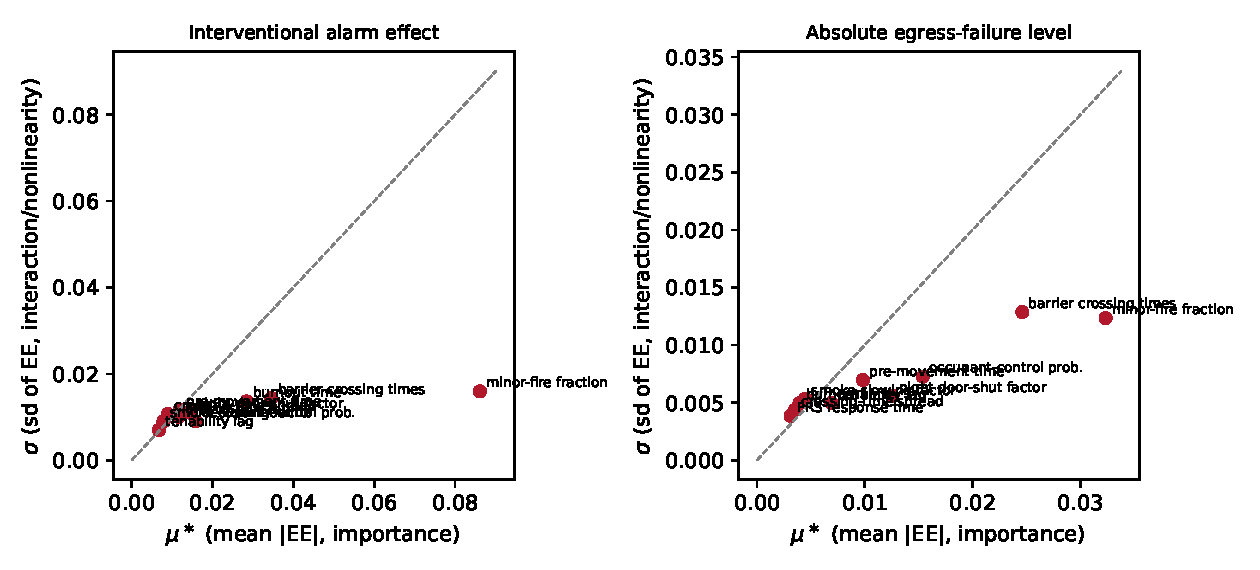
\includegraphics[width=0.92\linewidth]{figures/morris.pdf}
  \caption{Morris elementary-effects screening of the ten \emph{eng} simulator
  assumptions, for the interventional alarm effect (left) and the absolute
  evacuation-failure level (right). Each point is one assumption; $\mu^\ast$
  (horizontal) is its importance and $\sigma$ (vertical) its
  interaction/nonlinearity. The minor-fire fraction and crossing-time scale are
  the stiff directions for both outputs; burnout time is additionally stiff for
  the alarm effect (left) but sloppy for the absolute level (right). The
  interventional alarm effect stays protective and the archetype ranking fixed
  (Kendall $\tau\ge0.90$) across all $220$ design points.}
  \label{fig:morris}
\end{figure}
